\documentclass[11pt, a4paper]{report}
\usepackage[dvipsnames]{xcolor}
\usepackage{graphicx} % Required for inserting images
\usepackage{amsmath}
\usepackage[super]{natbib}
\usepackage[colorlinks=true, citecolor=blue]{hyperref}
\usepackage[margin=3cm]{geometry}

\begin{document}
% COVER PAGE
\thispagestyle{empty}

\vfill
\begin{center}
    \centering
    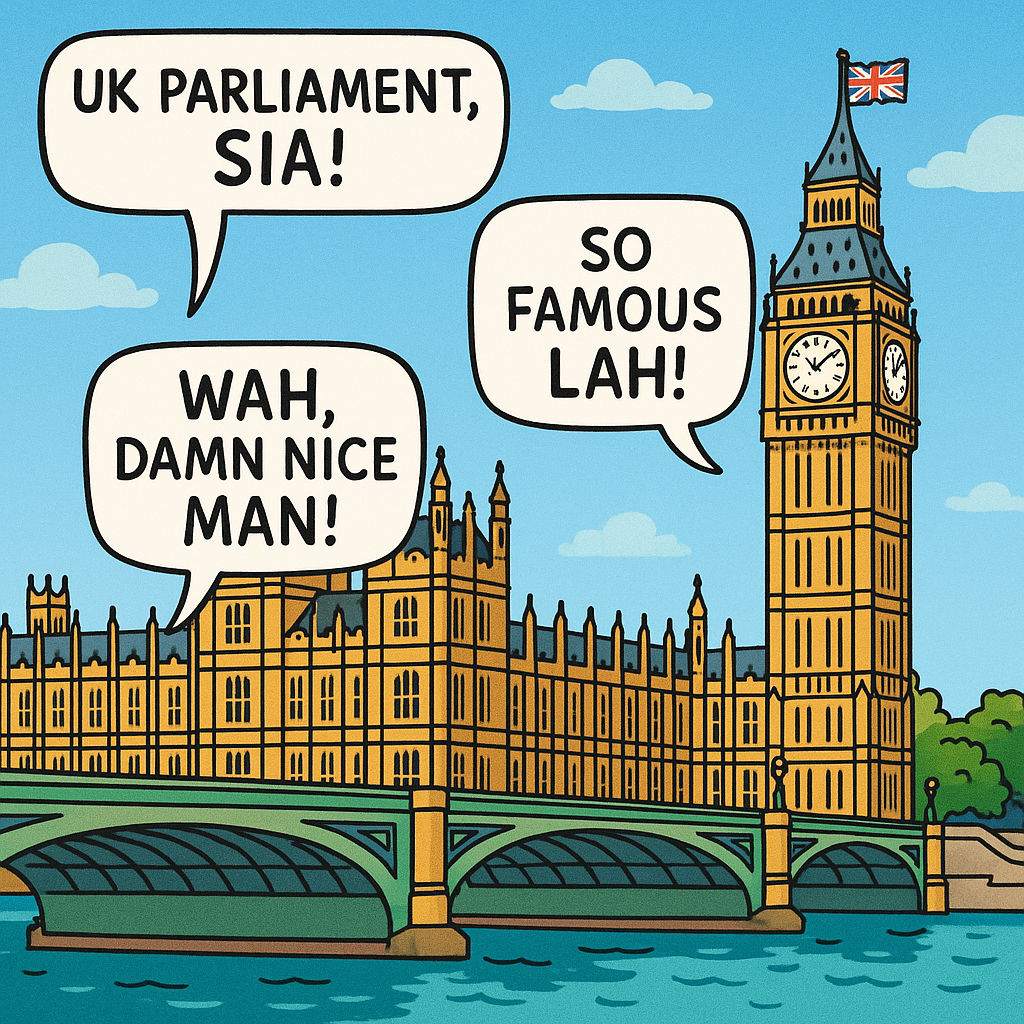
\includegraphics[width=\textwidth]{Cover/Figures/cover.png}
    % {\LARGE \emph{Spirals, defects, rolls and bands;} \\ Transitional Rayleigh-B\'{e}nard Poiseuille flows \\ Transitional sheared thermoconvective flows \\ using spectral/\emph{hp} element methods}

    \vspace{1cm}

    {\LARGE \emph{Oi}, jyyyuuu alroight?!}

    \rule{11cm}{1pt}
    \vspace{1cm}
    % Add paragraph space after/before vspace for vspace to work

    \textsc{\large Cambridge University Press} \\
    \textsc{\large Department of linguistics leh} \\
    
    \vspace{2cm}
    \emph{Author:} Chi Hin Chan \\ % Your name} 
    \emph{Honorary Authors:} Sandra Poecshmann % Your name} \\
    % ~
    % \begin{minipage}{0.4\textwidth}
    %     \begin{flushright}
    %         \emph{Supervisor:} \\
    %         Professor Spencer J. Sherwi
    %         % Uncomment the following lines if there's a co-supervisor
    %         \\[1.2em] % Supervisor's Name
    %         \emph{Co-Supervisor} \\
    %         Professor Yongyun Hwang % second marker's name
    %     \end{flushright}
    % \end{minipage}\\[3cm]
    % \makeatother
    % \emph{Ph.D. Thesis}
\end{center}

% \vfill
% 
\clearpage


\chapter{The basics}
One of the main motivations of writing this two-page book is to document the array of fancy vocabulary spoken in the UK, necessary for navigating (surviving) the social life here (or Singapore) - if you desire one.
Of course, this book would not be useful for you if you prefer the life of a \textit{hikikomori} \footnote{A severe form of social withdrawal}, but sorry no refunds.
I have lived in the UK for 3 years, and have taken some effort to the understand the beautiful nauced English language sufficiently.
As you might have already guessed from my name, I grew up in Singapore and became $200\%$ proficient in the art of Singlish after reciting the pledge for more than 10 years of my life, \textit{wa wayang leh}.
You can only imagine the awkward stares I received when I said that `\emph{wa I'm damm shagged man}' to my non-Singaporean (\textit{Malaysia also can}) friends.

If you are starting your life in the UK (or Singapore), I hope that you will find this list of translation useful for navigating the some of the awkward conversations I had.
In the following incomplete list (i.e. work in proogress), we will outline some of the basic slangs commonly spoken in both countries.
As you might have already noticed, the \textit{italised} words refer to \textit{Singlish} vocabulary, and the words that come after the hyphen `-' are in English,

\begin{enumerate}
    \item \textit{OI!} - You alright (or, DYUU OLRIOIGHT),
    \item \textit{You know hor} - Do you know what I mean (or, JEANETTE AMIN),
    \item \textit{Shag sia} - I'm knackered,
    \item \textit{Siao ah} - Shocking!
    \item \textit{Fun sia} - Oh its mad fun bruv,
    \item \textit{Jialat} - I'm not having it.
    \item \textit{Sibei Jialat} - I'm not having \textbf{ANY} of it.
    \item \textit{Stun like vegetable} - I'm shocked.
    \item \textit{You know horr} - Oh sorry, are you informed of.. 
\end{enumerate}

When it doubt, begin your sentences with `Oh sorry'! \textbf{Good luck!!}

\chapter{Becasue a single chapter isn't sufficient}
\begin{enumerate}
    \item \textit{Auntie one Kopi please} - Can I have a latte please, thank you!
    \item \textit{Chin chai} - Whatever..
    \item \textit{Hot sia} - It's \textbf{BOILLING} init!
    \item \textit{Siao ah} - THAT'S CRIMINAL!
    \item \textit{Malu} - A disgrace
\end{enumerate}

\newpage

\chapter{Entries from Google response}

The entries below are fetched from Google sheets.
\begin{enumerate}
\item \textit{Malu} - Disgraceful! (Ch)
\item \textit{Shag sia test} - I'm knackered test (Ch)
\item \textit{Oi} - you alright (Ch)
\item \textit{Sian} - I'm not having it test (Ch)
\item \textit{test} - test (test)
\end{enumerate}


\end{document}
